% Seminar 2: Distribuții Stabile
% Statistica Piețelor Financiare
% Program de licență, Academia de Studii Economice din București

\documentclass[9pt, aspectratio=169, t]{beamer}

% Asigură încadrarea conținutului pe diapozitive
\setbeamersize{text margin left=8mm, text margin right=8mm}

%=============================================================================
% CONFIGURARE TEMĂ ȘI STIL
%=============================================================================
\usetheme{default}

% Color Palette
\definecolor{MainBlue}{RGB}{26, 58, 110}
\definecolor{AccentBlue}{RGB}{26, 58, 110}
\definecolor{IDAred}{RGB}{205, 0, 0}
\definecolor{DarkGray}{RGB}{51, 51, 51}
\definecolor{MediumGray}{RGB}{128, 128, 128}
\definecolor{LightGray}{RGB}{248, 248, 248}
\definecolor{VeryLightGray}{RGB}{235, 235, 235}
\definecolor{KeynoteGray}{RGB}{218, 218, 218}
\definecolor{SectionGray}{RGB}{120, 120, 120}
\definecolor{FooterGray}{RGB}{100, 100, 100}
\definecolor{Crimson}{RGB}{220, 53, 69}
\definecolor{Forest}{RGB}{46, 125, 50}
\definecolor{Amber}{RGB}{181, 133, 63}
\definecolor{Orange}{RGB}{230, 126, 34}
\definecolor{Purple}{RGB}{142, 68, 173}

% Gradient background (background canvas ensures it works on fragile frames too)
\setbeamertemplate{background canvas}{%
    \begin{tikzpicture}[remember picture, overlay]
        \shade[shading=axis, shading angle=315,
        top color=white, bottom color=KeynoteGray]
        (current page.south west) rectangle (current page.north east);
    \end{tikzpicture}%
}

\setbeamercolor{palette primary}{bg=MainBlue, fg=white}
\setbeamercolor{palette secondary}{bg=MainBlue!85, fg=white}
\setbeamercolor{palette tertiary}{bg=MainBlue!70, fg=white}
\setbeamercolor{structure}{fg=MainBlue}
\setbeamercolor{title}{fg=IDAred}
\setbeamercolor{frametitle}{fg=IDAred, bg=}
\setbeamercolor{block title}{bg=MainBlue, fg=white}
\setbeamercolor{block body}{bg=VeryLightGray, fg=DarkGray}
\setbeamercolor{block title alerted}{bg=Crimson, fg=white}
\setbeamercolor{block body alerted}{bg=Crimson!8, fg=DarkGray}
\setbeamercolor{block title example}{bg=Forest, fg=white}
\setbeamercolor{block body example}{bg=Forest!8, fg=DarkGray}
\setbeamercolor{item}{fg=MainBlue}

% Culori subsol
\setbeamercolor{author in head/foot}{fg=FooterGray, bg=}
\setbeamercolor{title in head/foot}{fg=FooterGray, bg=}
\setbeamercolor{date in head/foot}{fg=FooterGray, bg=}
\setbeamercolor{section in head/foot}{fg=FooterGray, bg=}
\setbeamercolor{subsection in head/foot}{fg=FooterGray, bg=}

% Stiluri marcatori
\setbeamertemplate{itemize item}{\color{MainBlue}$\boxdot$}
\setbeamertemplate{itemize subitem}{\color{MainBlue}$\blacktriangleright$}
\setbeamertemplate{itemize subsubitem}{\color{MainBlue}\tiny$\bullet$}
\setbeamertemplate{itemize/enumerate body begin}{\normalsize}
\setbeamertemplate{itemize/enumerate subbody begin}{\normalsize}

% Spațiere elemente
\setlength{\leftmargini}{10pt}
\setlength{\leftmarginii}{10pt}
\makeatletter
\def\@listi{\leftmargin\leftmargini \topsep 0pt \parsep 0pt \itemsep 0pt}
\def\@listii{\leftmargin\leftmarginii \topsep 0pt \parsep 0pt \itemsep 0pt}
\makeatother

\setbeamertemplate{navigation symbols}{}

%=============================================================================
% ANTET PERSONALIZAT
%=============================================================================
\setbeamertemplate{headline}{%
    \vskip10pt%
    \hbox to \paperwidth{%
        \hskip0.5cm%
        {\small\color{FooterGray}\renewcommand{\hyperlink}[2]{##2}\insertsectionhead}%
        \hfill%
        \textcolor{FooterGray}{\small\insertframenumber}%
        \hskip0.5cm%
    }%
    \vskip4pt%
    {\color{FooterGray}\hrule height 0.4pt}%
}

%=============================================================================
% SUBSOL PERSONALIZAT
%=============================================================================
\usepackage{fontawesome5}

\setbeamertemplate{footline}{%
    {\color{FooterGray}\hrule height 0.4pt}%
    \vskip4pt%
    \hbox to \paperwidth{%
        \hskip0.5cm%
        \textcolor{FooterGray}{\small Statistica Piețelor Financiare --- Seminar}%
        \hfill%
        \raisebox{-0.1em}{%
            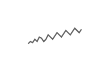
\begin{tikzpicture}[x=0.08em, y=0.08em, line width=0.4pt]
                \draw[FooterGray] (0,3) -- (1,4) -- (2,3.5) -- (3,5) -- (4,4) -- (5,6) -- (6,5.5) -- (7,4) -- (8,5) -- (9,7) -- (10,6) -- (11,5) -- (12,6.5) -- (13,8) -- (14,7) -- (15,6) -- (16,7.5) -- (17,9) -- (18,8) -- (19,7) -- (20,8.5) -- (21,10) -- (22,9) -- (23,8) -- (24,9.5);
            \end{tikzpicture}%
        }%
        \hskip0.5cm%
    }%
    \vskip6pt%
}

%=============================================================================
% PACHETE
%=============================================================================
\usepackage[utf8]{inputenc}
\usepackage[T1]{fontenc}
\usepackage{amsmath, amssymb, amsthm}
\usepackage{mathtools}
\usepackage{bm}
\usepackage{tikz}
\usetikzlibrary{arrows.meta, positioning, shapes, calc, decorations.pathreplacing, shadings}
\usepackage{booktabs}
\usepackage{multirow}
\usepackage{array}
\usepackage{graphicx}
\usepackage{hyperref}
\usepackage{colortbl}
\usepackage{listings}
\lstset{language=Python, basicstyle=\ttfamily\scriptsize, keywordstyle=\color{MainBlue}\bfseries,
  commentstyle=\color{Forest}, stringstyle=\color{Crimson}, breaklines=true,
  frame=none, backgroundcolor=\color{VeryLightGray}, xleftmargin=2mm}
\hypersetup{colorlinks=true, linkcolor=MainBlue, urlcolor=MainBlue}
\graphicspath{{../../logos/}{../../charts/}{../../photos/}}
\hfuzz=2pt
\vfuzz=2pt

%=============================================================================
% COMANDA QUANTLET
%=============================================================================
\newcommand{\quantlet}[2]{%
    \hfill\href{#2}{%
        \raisebox{-0.15em}{
\includegraphics[height=0.7em]{ql_logo.png}}%
        \textcolor{MainBlue}{\tiny\ #1}%
    }%
}

%=============================================================================
% PAGINĂ TITLU PERSONALIZATĂ
%=============================================================================
\defbeamertemplate*{title page}{hybrid}[1][]
{
    \vspace{0.2cm}
    \begin{center}
        \href{https://www.ase.ro}{
\includegraphics[height=1.0cm]{ase_logo.png}}\hspace{0.3cm}%
        \href{https://theida.net}{
\includegraphics[height=1.0cm]{ida_logo.png}}\hspace{0.3cm}%
        \href{https://blockchain-research-center.com}{
\includegraphics[height=1.0cm]{brc_logo.png}}\hspace{0.3cm}%
        \href{https://www.ai4efin.ase.ro}{
\includegraphics[height=1.0cm]{ai4efin_logo.png}}\hspace{0.3cm}%
        \href{https://ipe.ro/new}{
\includegraphics[height=1.0cm]{acad_logo.png}}\hspace{0.3cm}%
        \href{https://www.digital-finance-msca.com}{
\includegraphics[height=1.0cm]{msca_logo.png}}%
    \end{center}

    \vspace{0.6cm}

    \begin{center}
        \begin{minipage}{0.1\textwidth}
            \centering
            \href{https://quantlet.com}{
\includegraphics[height=1.1cm]{ql_logo.png}}
        \end{minipage}%
        \begin{minipage}{0.78\textwidth}
            \centering
            {\LARGE\bfseries\usebeamercolor[fg]{title}\inserttitle}

            \vspace{0.3cm}

            {\usebeamerfont{subtitle}\usebeamercolor[fg]{title}\insertsubtitle}
        \end{minipage}%
        \begin{minipage}{0.1\textwidth}
            \centering
            \href{https://quantinar.com}{
\includegraphics[height=1.1cm]{qr_logo.png}}
        \end{minipage}
    \end{center}

    \vspace{0.6cm}

    \hspace{0.5cm}\begin{minipage}[t]{0.9\textwidth}
        \raggedright{\usebeamerfont{author}\insertauthor}
    \end{minipage}

    \vspace{0.3cm}

    \hspace{0.5cm}\begin{minipage}[t]{0.9\textwidth}
        \raggedright\small\insertinstitute
    \end{minipage}
}

%=============================================================================
% MEDII PENTRU TEOREME
%=============================================================================
\theoremstyle{definition}
\setbeamertemplate{theorems}[numbered]
\newtheorem{defn}{Definiție}
\newtheorem{thm}{Teoremă}
\newtheorem{prop}{Propoziție}
\newtheorem{rmk}{Observație}

%=============================================================================
% CENTRED MINIPAGE
%=============================================================================
\newenvironment{cminipage}[1]{%
    \par\noindent\hfill\begin{minipage}{#1}\ignorespaces
}{%
    \end{minipage}\hfill\null\par
}

%=============================================================================
% COMENZI PERSONALIZATE
%=============================================================================
\newcommand{\E}{\mathbb{E}}
\newcommand{\Var}{\text{Var}}
\newcommand{\Cov}{\text{Cov}}
\newcommand{\Corr}{\text{Corr}}
\newcommand{\R}{\mathbb{R}}
\newcommand{\N}{\mathbb{N}}
\newcommand{\Z}{\mathbb{Z}}
\newcommand{\B}{\mathbf{B}}
\newcommand{\imark}{\textcolor{MainBlue}{\textbullet}}
\newcommand{\RMSE}{\text{RMSE}}
\newcommand{\MAE}{\text{MAE}}
\newcommand{\MAPE}{\text{MAPE}}

%=============================================================================
% INFORMAȚII TITLU
%=============================================================================
\title[Statistica Piețelor Financiare]{Statistica Piețelor Financiare}
\subtitle{Seminar 2: Distribuții Stabile}
\author[D.T. Pele, A. Amza]{Daniel Traian PELE \\ Antoaneta Amza}
\institute{Academia de Studii Economice din București\\
IDA Institute Digital Assets\\
Blockchain Research Center\\
AI4EFin Artificial Intelligence for Energy Finance\\
Academia Română, Institutul de Prognoză Economică\\
MSCA Digital Finance}
\date{}

\begin{document}

%=============================================================================
% PAGINA DE TITLU
%=============================================================================
{
\setbeamertemplate{headline}{}
\setbeamertemplate{footline}{}
\begin{frame}[noframenumbering]
    \titlepage
\end{frame}
}

%=============================================================================
% OBIECTIVE
%=============================================================================
\section{Obiective}

\begin{frame}{Obiective de învățare}
\begin{columns}[T]
\begin{column}{0.55\textwidth}
\begin{block}{La finalul seminarului veți putea:}
\begin{itemize}
    \item Verifica proprietatea de stabilitate pentru Gaussiană și Cauchy
    \item Calcula funcția caracteristică a unei distribuții stabile
    \item Analiza momentele și comportamentul cozilor
    \item Estima parametrii unei distribuții stabile (McCulloch, MLE)
    \item Compara VaR: Gaussiană vs Stabilă vs Empiric
    \item Implementa fit-ul stabil în Python
\end{itemize}
\end{block}
\end{column}
\begin{column}{0.42\textwidth}
\begin{center}
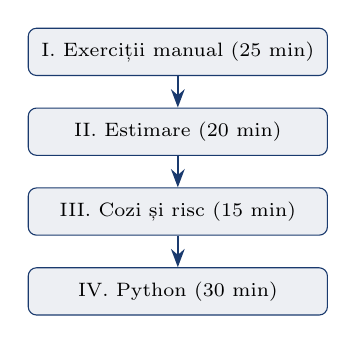
\begin{tikzpicture}[
    node distance=0.4cm,
    every node/.style={font=\scriptsize, align=center},
    phase/.style={draw=MainBlue, fill=MainBlue!8, rounded corners=3pt,
                  minimum width=3.8cm, minimum height=0.6cm}
]
\node[phase] (p1) {I. Exerciții manual (25 min)};
\node[phase, below=of p1] (p2) {II. Estimare (20 min)};
\node[phase, below=of p2] (p3) {III. Cozi și risc (15 min)};
\node[phase, below=of p3] (p4) {IV. Python (30 min)};
\draw[-{Stealth}, MainBlue, thick] (p1) -- (p2);
\draw[-{Stealth}, MainBlue, thick] (p2) -- (p3);
\draw[-{Stealth}, MainBlue, thick] (p3) -- (p4);
\end{tikzpicture}
\end{center}
\end{column}
\end{columns}
\end{frame}

%=============================================================================
% PARTEA I: EXERCIȚII MANUAL
%=============================================================================
\section{Partea I: Exerciții manual}

\begin{frame}{Exercițiul 1: Verificarea stabilității --- Cazul Gaussian}
\begin{block}{Problemă}
Fie $X_1, X_2$ variabile i.i.d. $\sim \mathcal{N}(0, 1)$. Arătați că
$a X_1 + b X_2 \stackrel{d}{=} c X + d$ pentru $a=3, b=4, c=5$.
\end{block}

\begin{exampleblock}{Rezolvare}
Dacă $X_1 \sim \mathcal{N}(0, 1)$, atunci $aX_1 \sim \mathcal{N}(0, a^2)$ și $bX_2 \sim \mathcal{N}(0, b^2)$.

Suma: $aX_1 + bX_2 \sim \mathcal{N}(0, a^2 + b^2) = \mathcal{N}(0, 9 + 16) = \mathcal{N}(0, 25)$.

Deci $c = \sqrt{a^2 + b^2} = \sqrt{25} = 5$ și $d = 0$.

\vspace{0.2cm}
\textbf{Concluzie:} Distribuția normală este stabilă cu $\alpha = 2$. Proprietatea de stabilitate se reduce la regula adunării varianțelor.
\end{exampleblock}
\end{frame}

\begin{frame}{Exercițiul 1 cont.: Cazul Cauchy + Tabel comparativ}
\begin{columns}[T]
\begin{column}{0.48\textwidth}
\begin{block}{Cazul Cauchy ($\alpha = 1$)}
Fie $X_1, X_2 \sim \text{Cauchy}(0,1)$ i.i.d.

$aX_1 + bX_2 \sim \text{Cauchy}(0, a+b)$

Pentru $a=3, b=4$: $c = a + b = 7$, $d = 0$.

\vspace{0.2cm}
\textbf{Notă:} La Cauchy, scara se adună \textit{liniar}, nu pătratic!
\end{block}
\end{column}
\begin{column}{0.48\textwidth}
\begin{block}{Regula generală}
Pentru $S(\alpha, \beta, \gamma, \delta)$:
$$c^\alpha = a^\alpha + b^\alpha$$

\vspace{0.2cm}
\renewcommand{\arraystretch}{1.3}
\begin{tabular}{lccc}
\toprule
& $\alpha$ & Regulă & $c$ \\
\midrule
Gaussian & 2 & $c^2 = a^2+b^2$ & 5 \\
Cauchy & 1 & $c = a+b$ & 7 \\
$S(1.5)$ & 1.5 & $c^{1.5} = a^{1.5}+b^{1.5}$ & 6.19 \\
\bottomrule
\end{tabular}
\end{block}
\end{column}
\end{columns}
\end{frame}

\begin{frame}{Exercițiul 2: Funcția caracteristică}
\begin{block}{Problemă}
Calculați $\varphi_X(t)$ pentru $X \sim S(1.5, 0.3, 1, 0)$ la $t = 1$.
\end{block}

\begin{exampleblock}{Rezolvare}
Funcția caracteristică a distribuției stabile:
$$\log \varphi_X(t) = -|t|^\alpha \left[1 - i\beta\,\text{sgn}(t)\tan\frac{\pi\alpha}{2}\right] + i\delta t$$

Pentru $\alpha = 1.5$, $\beta = 0.3$, $\gamma = 1$, $\delta = 0$, $t = 1$:
$$\log \varphi_X(1) = -|1|^{1.5}\left[1 - i \cdot 0.3 \cdot 1 \cdot \tan\frac{3\pi}{4}\right]$$
$$= -1 \cdot [1 - i \cdot 0.3 \cdot (-1)] = -1 - 0.3i$$

Deci:
$$\varphi_X(1) = e^{-1 - 0.3i} = e^{-1}(\cos 0.3 - i\sin 0.3) \approx 0.351 - 0.109i$$
$$|\varphi_X(1)| = e^{-1} \approx 0.368$$
\end{exampleblock}
\end{frame}

\begin{frame}{Exercițiul 3: Momente și cozi}
\begin{block}{Problemă}
Un analist financiar modelează randamentele zilnice cu $S(1.7, -0.2, 0.01, 0.0005)$. Care momente există? Ce implică pentru managementul riscului?
\end{block}

\begin{exampleblock}{Rezolvare}
\begin{columns}[T]
\begin{column}{0.48\textwidth}
\textbf{Existența momentelor:}
\begin{itemize}
    \item $\E[|X|^p] < \infty$ dacă și numai dacă $p < \alpha$
    \item $\alpha = 1.7 \Rightarrow$
    \begin{itemize}
        \item Media ($p=1$): \textcolor{Forest}{există} ($1 < 1.7$)
        \item Varianța ($p=2$): \textcolor{Crimson}{nu există} ($2 > 1.7$)
        \item Kurtosis ($p=4$): \textcolor{Crimson}{nu există}
    \end{itemize}
\end{itemize}
\end{column}
\begin{column}{0.48\textwidth}
\textbf{Implicații practice:}
\begin{itemize}
    \item $\beta = -0.2$: asimetrie negativă (risc la căderi)
    \item VaR Gaussian \textbf{subestimează} riscul real
    \item Probabilitatea unui eveniment $-5\sigma$:
    \begin{itemize}
        \item Normal: $\approx 3 \times 10^{-7}$ (1 la 3.5M zile)
        \item Stabil(1.7): $\approx 0.003$ (1 la 333 zile)
    \end{itemize}
    \item Sharpe ratio nu este definit riguros!
\end{itemize}
\end{column}
\end{columns}
\end{exampleblock}
\end{frame}

%=============================================================================
% PARTEA II: ESTIMARE
%=============================================================================
\section{Partea II: Estimare}

\begin{frame}{Metoda McCulloch --- Concept}
\begin{block}{Ideea principală}
Estimarea parametrilor $(\alpha, \beta, \gamma, \delta)$ din \textbf{cuantile} ale eșantionului.
\end{block}

\begin{columns}[T]
\begin{column}{0.48\textwidth}
\textbf{Statistici intermediare:}
$$v_\alpha = \frac{q_{0.95} - q_{0.05}}{q_{0.75} - q_{0.25}}$$
$$v_\beta = \frac{q_{0.95} + q_{0.05} - 2q_{0.50}}{q_{0.95} - q_{0.05}}$$

\vspace{0.2cm}
\begin{itemize}
    \item $v_\alpha$ măsoară \textit{greutatea cozilor} (tail thickness)
    \item $v_\beta$ măsoară \textit{asimetria}
\end{itemize}
\end{column}
\begin{column}{0.48\textwidth}
\textbf{Tabel de referință (selecție):}

\renewcommand{\arraystretch}{1.2}
\begin{tabular}{ccc}
\toprule
$v_\alpha$ & $\alpha$ & Interpretare \\
\midrule
2.44 & 2.0 & Gaussiană \\
2.62 & 1.9 & Aproape Gauss \\
3.04 & 1.7 & Cozi moderate \\
4.21 & 1.5 & Cozi grele \\
6.31 & 1.3 & Cozi foarte grele \\
\bottomrule
\end{tabular}
\end{column}
\end{columns}
\end{frame}

\begin{frame}{McCulloch --- Exercițiu rezolvat}
\begin{block}{Date numerice}
Din eșantionul de 2000 observații: $q_{0.05} = -3.42$, $q_{0.25} = -0.78$, $q_{0.50} = 0.05$, $q_{0.75} = 0.82$, $q_{0.95} = 3.61$.
\end{block}

\begin{exampleblock}{Rezolvare pas cu pas}
\textbf{Pasul 1: Calculăm $v_\alpha$}
$$v_\alpha = \frac{q_{0.95} - q_{0.05}}{q_{0.75} - q_{0.25}} = \frac{3.61 - (-3.42)}{0.82 - (-0.78)} = \frac{7.03}{1.60} = 4.39$$

\textbf{Pasul 2: Estimăm $\alpha$}
Din tabel: $v_\alpha = 4.39$ corespunde $\hat{\alpha} \approx 1.48$.

\textbf{Pasul 3: Calculăm $v_\beta$}
$$v_\beta = \frac{q_{0.95} + q_{0.05} - 2q_{0.50}}{q_{0.95} - q_{0.05}} = \frac{3.61 + (-3.42) - 2 \cdot 0.05}{7.03} = \frac{0.09}{7.03} \approx 0.013$$

\textbf{Pasul 4: Estimăm $\beta$}
$v_\beta \approx 0.013 \approx 0 \Rightarrow \hat{\beta} \approx 0$ (distribuție aproape simetrică).
\end{exampleblock}
\end{frame}

\begin{frame}[fragile]{Maximum Likelihood Estimation (MLE)}
\begin{block}{Procedura}
$$\hat{\theta}_{MLE} = \arg\max_{\theta} \sum_{i=1}^{n} \log f(x_i; \alpha, \beta, \gamma, \delta)$$
\end{block}

\begin{columns}[T]
\begin{column}{0.48\textwidth}
\textbf{Provocări:}
\begin{itemize}
    \item PDF-ul nu are formă închisă (în general)
    \item Trebuie evaluare numerică prin FFT
    \item Funcția de verosimilitate nu e convexă
    \item Convergență lentă pentru $\alpha$ mic
\end{itemize}
\end{column}
\begin{column}{0.48\textwidth}
\textbf{Avantaje:}
\begin{itemize}
    \item Cea mai eficientă estimare asimptotic
    \item Intervale de încredere standard
    \item Implementare modernă: \texttt{scipy.stats.levy\_stable.fit()}
\end{itemize}

\vspace{0.2cm}
\textbf{One-liner Python:}
\begin{lstlisting}
from scipy.stats import levy_stable
a, b, loc, sc = levy_stable.fit(data)
\end{lstlisting}
\end{column}
\end{columns}
\end{frame}

\begin{frame}{Regresia Koutrouvelis}
\begin{block}{Metoda în 2 etape}
Se utilizează funcția caracteristică empirică (ECF).
\end{block}

\textbf{Etapa 1:} Estimarea $\alpha$ și $\gamma$ prin regresie liniară:
$$\log\left(-\log|\hat{\varphi}_n(t)|^2\right) = \log(2\gamma^\alpha) + \alpha \log|t|$$
Regresie $Y = a + bX$ cu $Y_k = \log(-\log|\hat{\varphi}_n(t_k)|^2)$ și $X_k = \log|t_k|$.

\vspace{0.3cm}
\textbf{Etapa 2:} Estimarea $\beta$ și $\delta$ prin regresie pe partea imaginară:
$$\arg[\hat{\varphi}_n(t)] = \delta t - \beta\gamma^\alpha \tan\frac{\pi\alpha}{2}\,\text{sgn}(t)|t|^\alpha$$

\vspace{0.2cm}
\begin{alertblock}{Avantaj}
Robustă numeric, nu necesită evaluarea PDF-ului, convergență rapidă.
\end{alertblock}
\end{frame}

%=============================================================================
% PARTEA III: COZI ȘI RISC
%=============================================================================
\section{Partea III: Cozi și risc}

\begin{frame}{Heavy tails --- Gaussiană vs Stabilă}
\quantlet{SFM\_ch2\_stable\_fit}{https://github.com/QuantLet/SFM}

\begin{block}{Tabel comparativ: Probabilitatea evenimentelor extreme}
\renewcommand{\arraystretch}{1.3}
\begin{center}
\begin{tabular}{lccc}
\toprule
\textbf{Eveniment} & \textbf{Gaussiană} & \textbf{Stabil($\alpha$=1.7)} & \textbf{Raport} \\
\midrule
$|X| > 3\sigma$ & $2.7 \times 10^{-3}$ & $1.9 \times 10^{-2}$ & $\approx 7\times$ \\
$|X| > 5\sigma$ & $5.7 \times 10^{-7}$ & $3.0 \times 10^{-3}$ & $\approx 5{,}000\times$ \\
$|X| > 10\sigma$ & $1.5 \times 10^{-23}$ & $5.2 \times 10^{-4}$ & $\approx 10^{19}\times$ \\
\bottomrule
\end{tabular}
\end{center}
\end{block}

\vspace{0.2cm}
\begin{alertblock}{Implicație practică}
Modelele Gaussiene subestimează dramatic riscul evenimentelor extreme. Un eveniment ``$10\sigma$'' pe care Gaussiana îl consideră practic imposibil apare o dată la $\sim$2{,}000 de zile ($\sim$8 ani) sub modelul stabil.
\end{alertblock}
\end{frame}

\begin{frame}{Exercițiul 4: VaR Gaussiană vs Stabilă}
\begin{block}{Problemă}
Portofoliu de 1{,}000{,}000 EUR. Randamente zilnice modelate cu $S(1.7, -0.2, 0.01, 0.0005)$. Comparați VaR la 1\%, 5\% și 0.1\%.
\end{block}

\begin{exampleblock}{Rezolvare}
\renewcommand{\arraystretch}{1.3}
\begin{center}
\begin{tabular}{lccc}
\toprule
\textbf{Nivel VaR} & \textbf{Gaussiană} & \textbf{Stabilă} & \textbf{Diferență} \\
\midrule
5\% & $-$16{,}449 EUR & $-$21{,}340 EUR & +30\% \\
1\% & $-$22{,}763 EUR & $-$39{,}870 EUR & +75\% \\
0.1\% & $-$30{,}091 EUR & $-$87{,}420 EUR & +190\% \\
\bottomrule
\end{tabular}
\end{center}

\vspace{0.2cm}
\textbf{Concluzie:} Cu cât nivelul de încredere este mai mare (cozi mai adânci), cu atât diferența Gaussiană vs Stabilă crește. La VaR 0.1\%, modelul stabil estimează pierderi de aproape \textbf{3 ori mai mari}.
\end{exampleblock}
\end{frame}

\begin{frame}{Comparație vizuală: Funcția de supraviețuire}
\quantlet{SFM\_ch2\_stable\_fit}{https://github.com/QuantLet/SFM}

\begin{center}
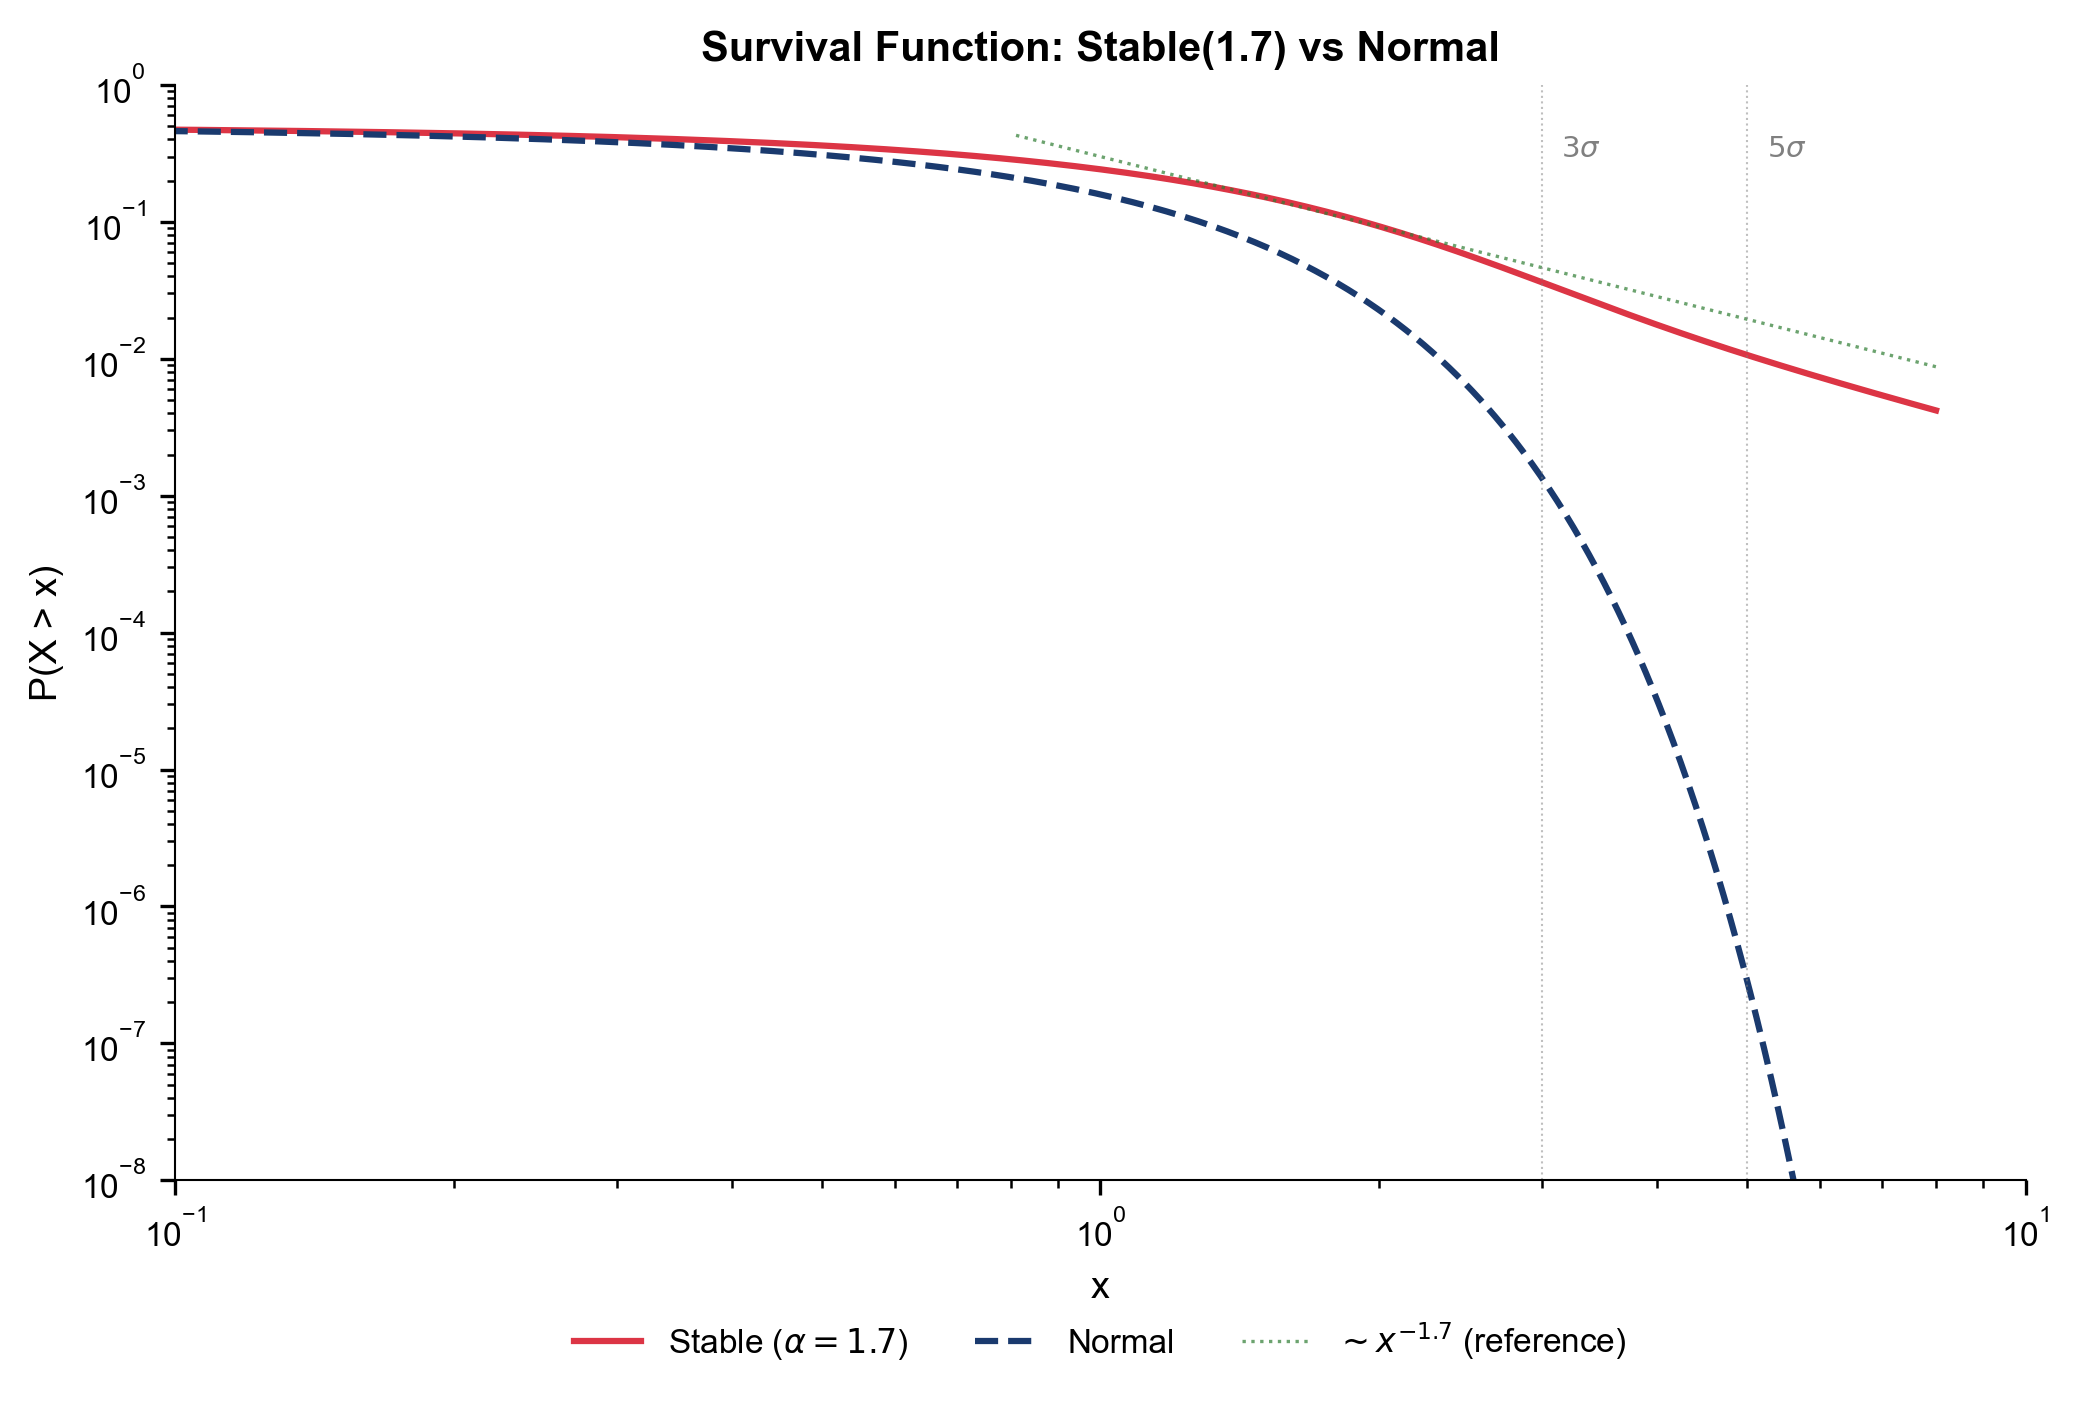
\includegraphics[width=0.75\textwidth]{ch2_tail_survival.png}
\end{center}

\vspace{-0.3cm}
\begin{itemize}
    \item Grafic log-log: funcția de supraviețuire $P(X > x)$
    \item Distribuția stabilă scade ca o \textbf{lege putere}: $P(X > x) \sim C_\alpha x^{-\alpha}$
    \item Distribuția normală scade \textbf{exponențial}: diferența crește rapid cu $x$
\end{itemize}
\end{frame}

%=============================================================================
% PARTEA IV: PYTHON
%=============================================================================
\section{Partea IV: Implementare Python}

\begin{frame}[fragile]{Simulare: Stable Distributions}
\begin{lstlisting}
import numpy as np
from scipy.stats import levy_stable
import matplotlib.pyplot as plt

alphas = [0.5, 1.0, 1.5, 2.0]
x = np.linspace(-8, 8, 1000)

fig, (ax1, ax2) = plt.subplots(1, 2, figsize=(14, 5))
colors = ['#DC3545', '#FF8C00', '#2E7D32', '#1A3A6E']
labels = ['alpha=0.5 (Levy)', 'alpha=1.0 (Cauchy)',
          'alpha=1.5', 'alpha=2.0 (Gaussian)']

for a, c, lab in zip(alphas, colors, labels):
    pdf = levy_stable.pdf(x, alpha=a, beta=0)
    ax1.plot(x, pdf, color=c, label=lab)
    ax2.semilogy(x, pdf, color=c, label=lab)

ax1.set_title('PDFs (linear)')
ax2.set_title('PDFs (log scale)')
for ax in [ax1, ax2]:
    ax.legend(loc='upper center',
              bbox_to_anchor=(0.5, -0.12), ncol=2)
plt.tight_layout()
\end{lstlisting}
\end{frame}

\begin{frame}[fragile]{Python: Stable Fit S\&P 500}
\begin{lstlisting}
import yfinance as yf
from scipy.stats import levy_stable, norm

sp500 = yf.download('^GSPC', start='2000-01-01',
                     end='2025-12-31')
returns = np.log(
    sp500['Close'] / sp500['Close'].shift(1)).dropna()

# Fit stable distribution
alpha, beta, loc, scale = levy_stable.fit(returns.values)
print(f"alpha={alpha:.3f}, beta={beta:.3f}")

# Fit normal
mu, sigma = norm.fit(returns.values)

# Compare on log-scale
x = np.linspace(returns.min()*1.2,
                returns.max()*1.2, 1000)
plt.hist(returns, bins=150, density=True,
         alpha=0.4, label='Data')
plt.semilogy(x, levy_stable.pdf(x, alpha, beta,
             loc, scale), label='Stable')
plt.semilogy(x, norm.pdf(x, mu, sigma),
             '--', label='Normal')
\end{lstlisting}
\end{frame}

\begin{frame}{Overlay PDF: Histogram + Stable + Normal (log-scale)}

\begin{center}
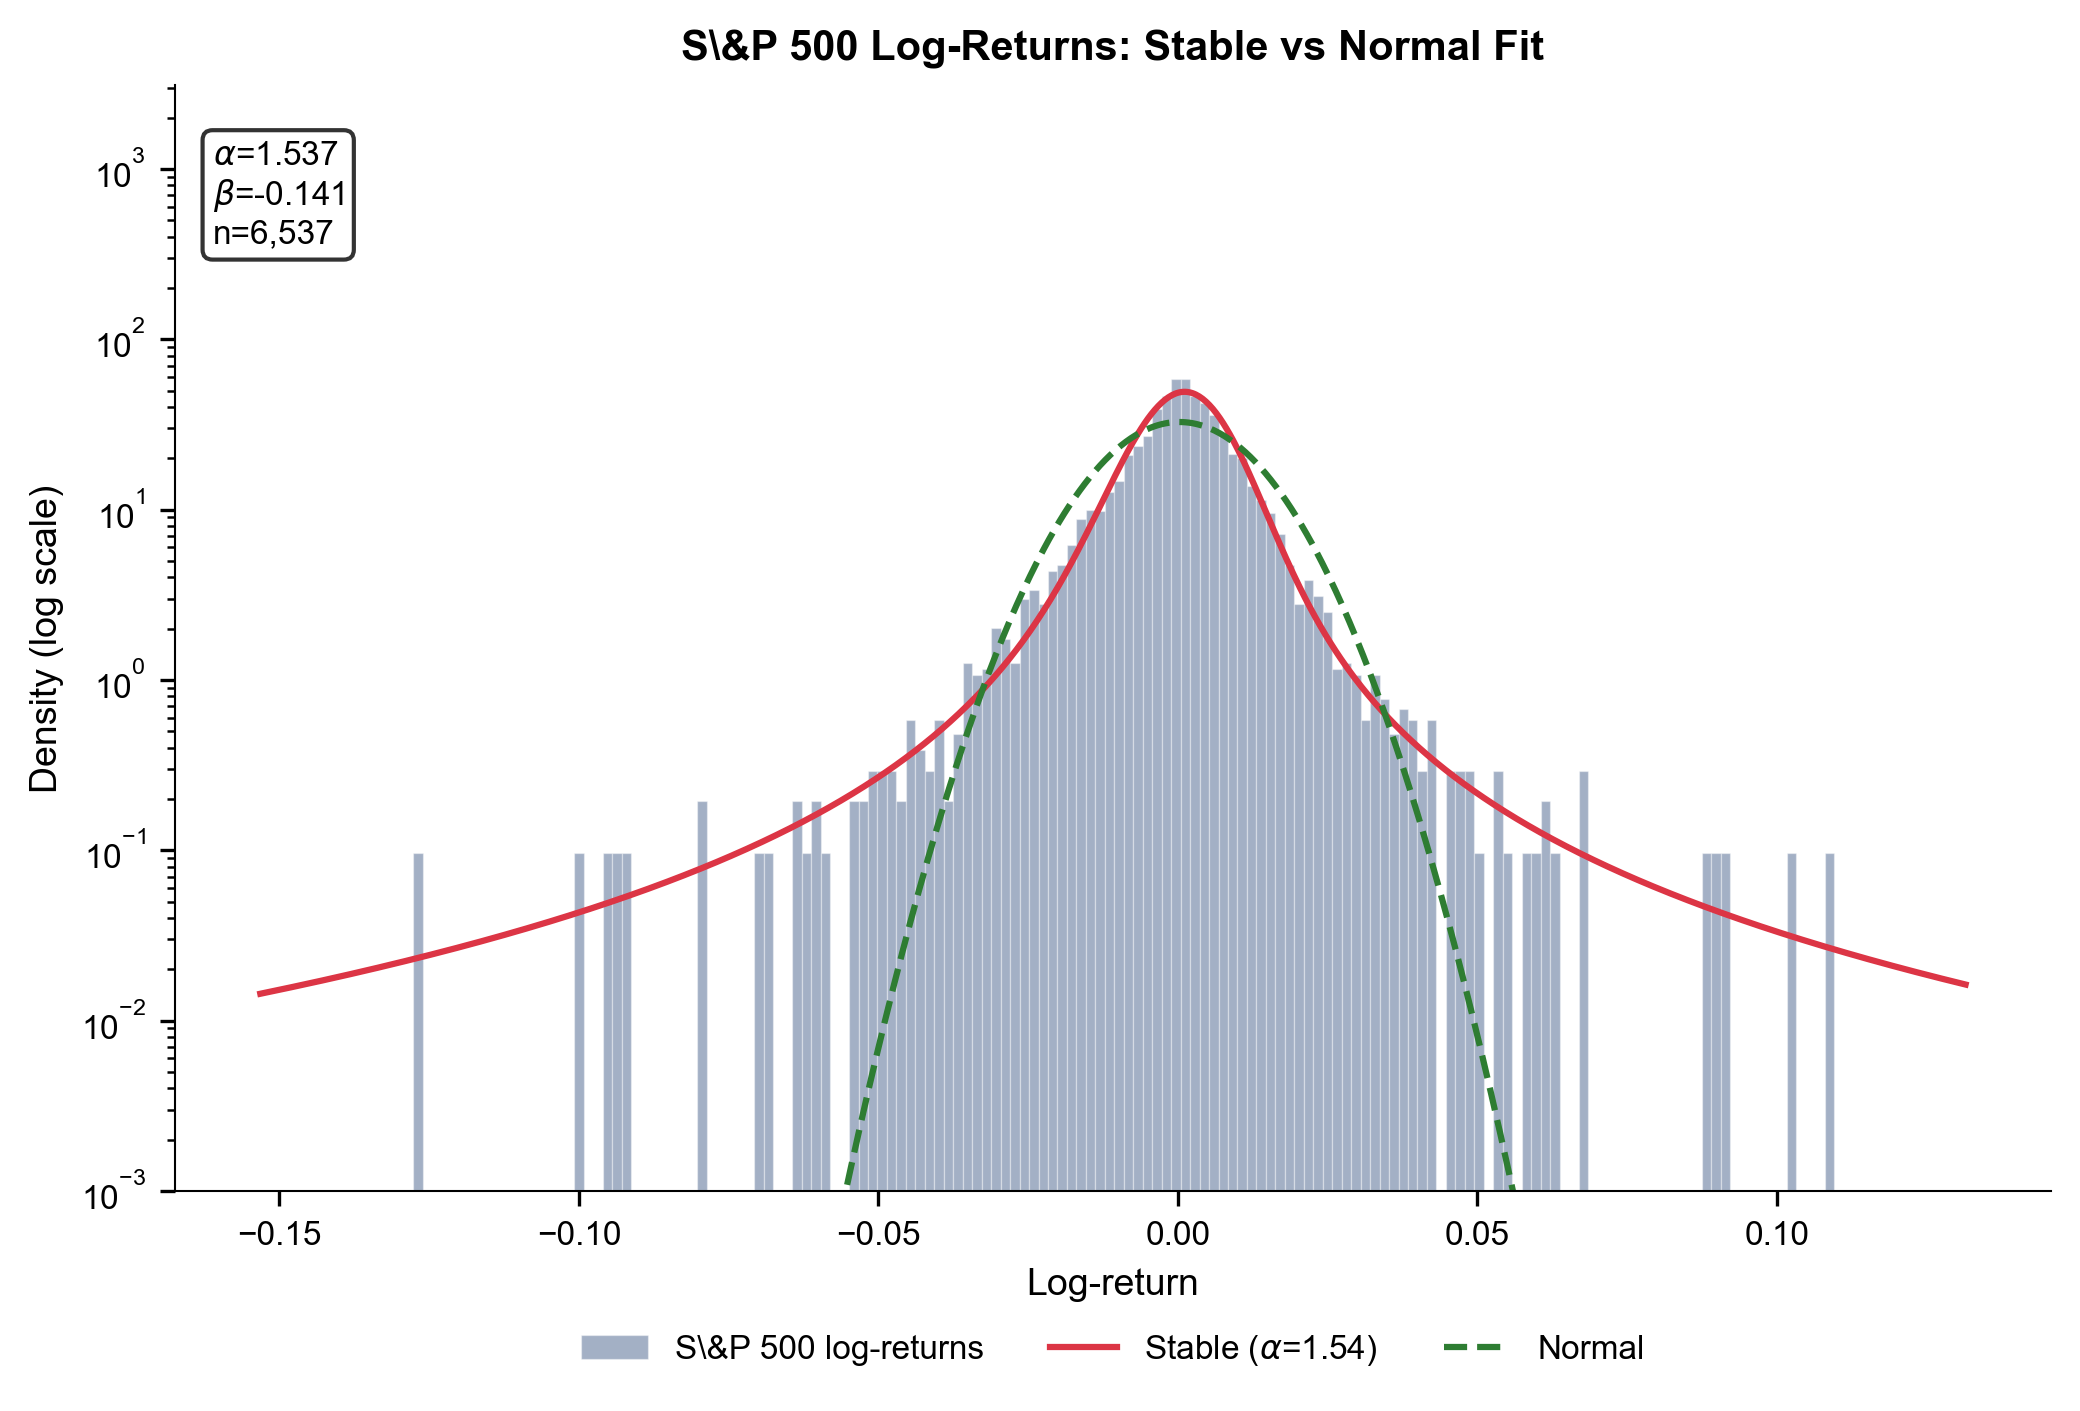
\includegraphics[width=0.78\textwidth]{ch2_sp500_stable_fit.png}
\end{center}

\vspace{-0.3cm}
\begin{itemize}
    \item Pe scară logaritmică, diferența în cozi este evidentă
    \item Distribuția stabilă captează \textbf{leptokurtoza} observată în date
    \item Normala subestimează probabilitățile din cozile distribuției
\end{itemize}
\end{frame}

\begin{frame}[fragile]{Python: VaR Comparison}

\begin{columns}[T]
\begin{column}{0.45\textwidth}
\begin{lstlisting}
# VaR comparison
levels = [0.01, 0.05, 0.001]
for cl in levels:
    var_s = levy_stable.ppf(
        cl, alpha, beta, loc, scale)
    var_n = norm.ppf(cl, mu, sigma)
    var_e = np.percentile(
        returns, cl*100)
    print(f"VaR {cl*100:.1f}%:")
    print(f"  Stable:    {var_s:.5f}")
    print(f"  Normal:    {var_n:.5f}")
    print(f"  Empirical: {var_e:.5f}")
\end{lstlisting}
\end{column}
\begin{column}{0.52\textwidth}
\begin{center}
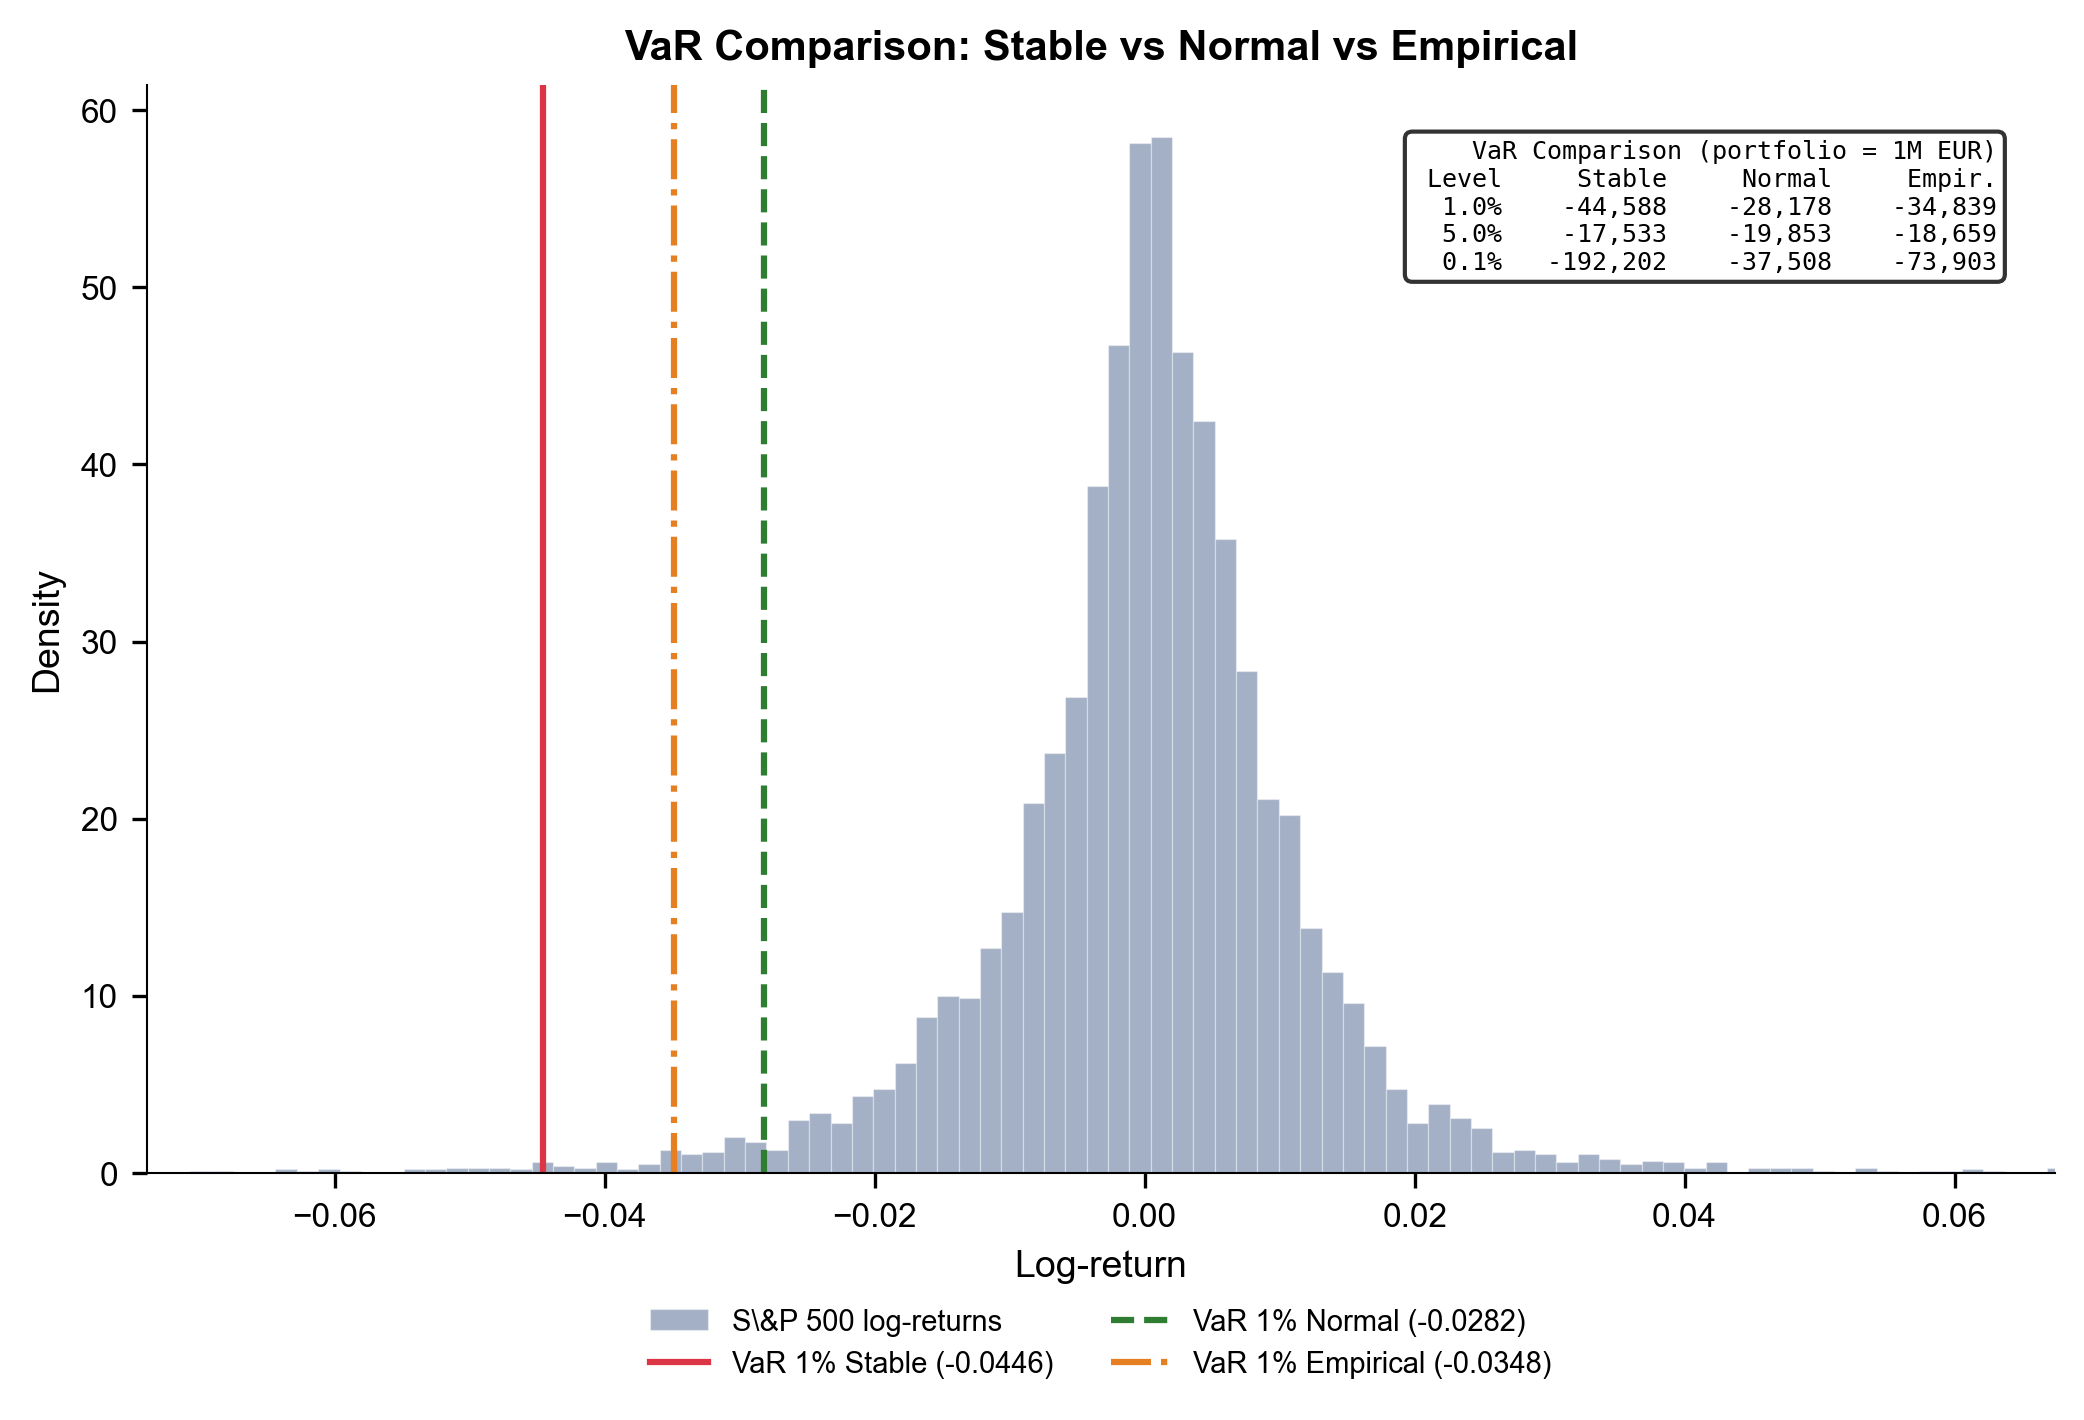
\includegraphics[width=\textwidth]{ch2_var_comparison.png}
\end{center}
\end{column}
\end{columns}
\end{frame}

\begin{frame}{Exercițiu AI: Prompt Engineering}
\begin{block}{Exercițiu}
Folosiți ChatGPT sau Claude pentru a genera cod Python care:
\end{block}

\begin{enumerate}
    \item Descarcă datele BTC-USD din ultimii 5 ani
    \item Fit-ează o distribuție stabilă pe log-randamentele zilnice
    \item Compară grafic PDF stabilă vs normală (log-scale)
    \item Calculează VaR la 1\% și 5\%
    \item Realizează un backtest: câte zile au depășit VaR-ul estimat?
\end{enumerate}

\vspace{0.3cm}
\begin{alertblock}{Prompt sugerat}
\textit{``Write Python code using scipy.stats.levy\_stable to fit a stable distribution to BTC-USD daily log-returns from yfinance. Plot histogram with stable and normal overlay on log-scale. Calculate VaR at 1\% and 5\% for both distributions and backtest against actual returns.''}
\end{alertblock}
\end{frame}

%=============================================================================
% STUDIU DE CAZ: S&P 500
%=============================================================================
\section{Studiu de caz: S\&P 500}

\begin{frame}{Histogram + Fit stabil vs Normal}
\quantlet{SFM\_ch2\_stable\_fit}{https://github.com/QuantLet/SFM}

\begin{center}
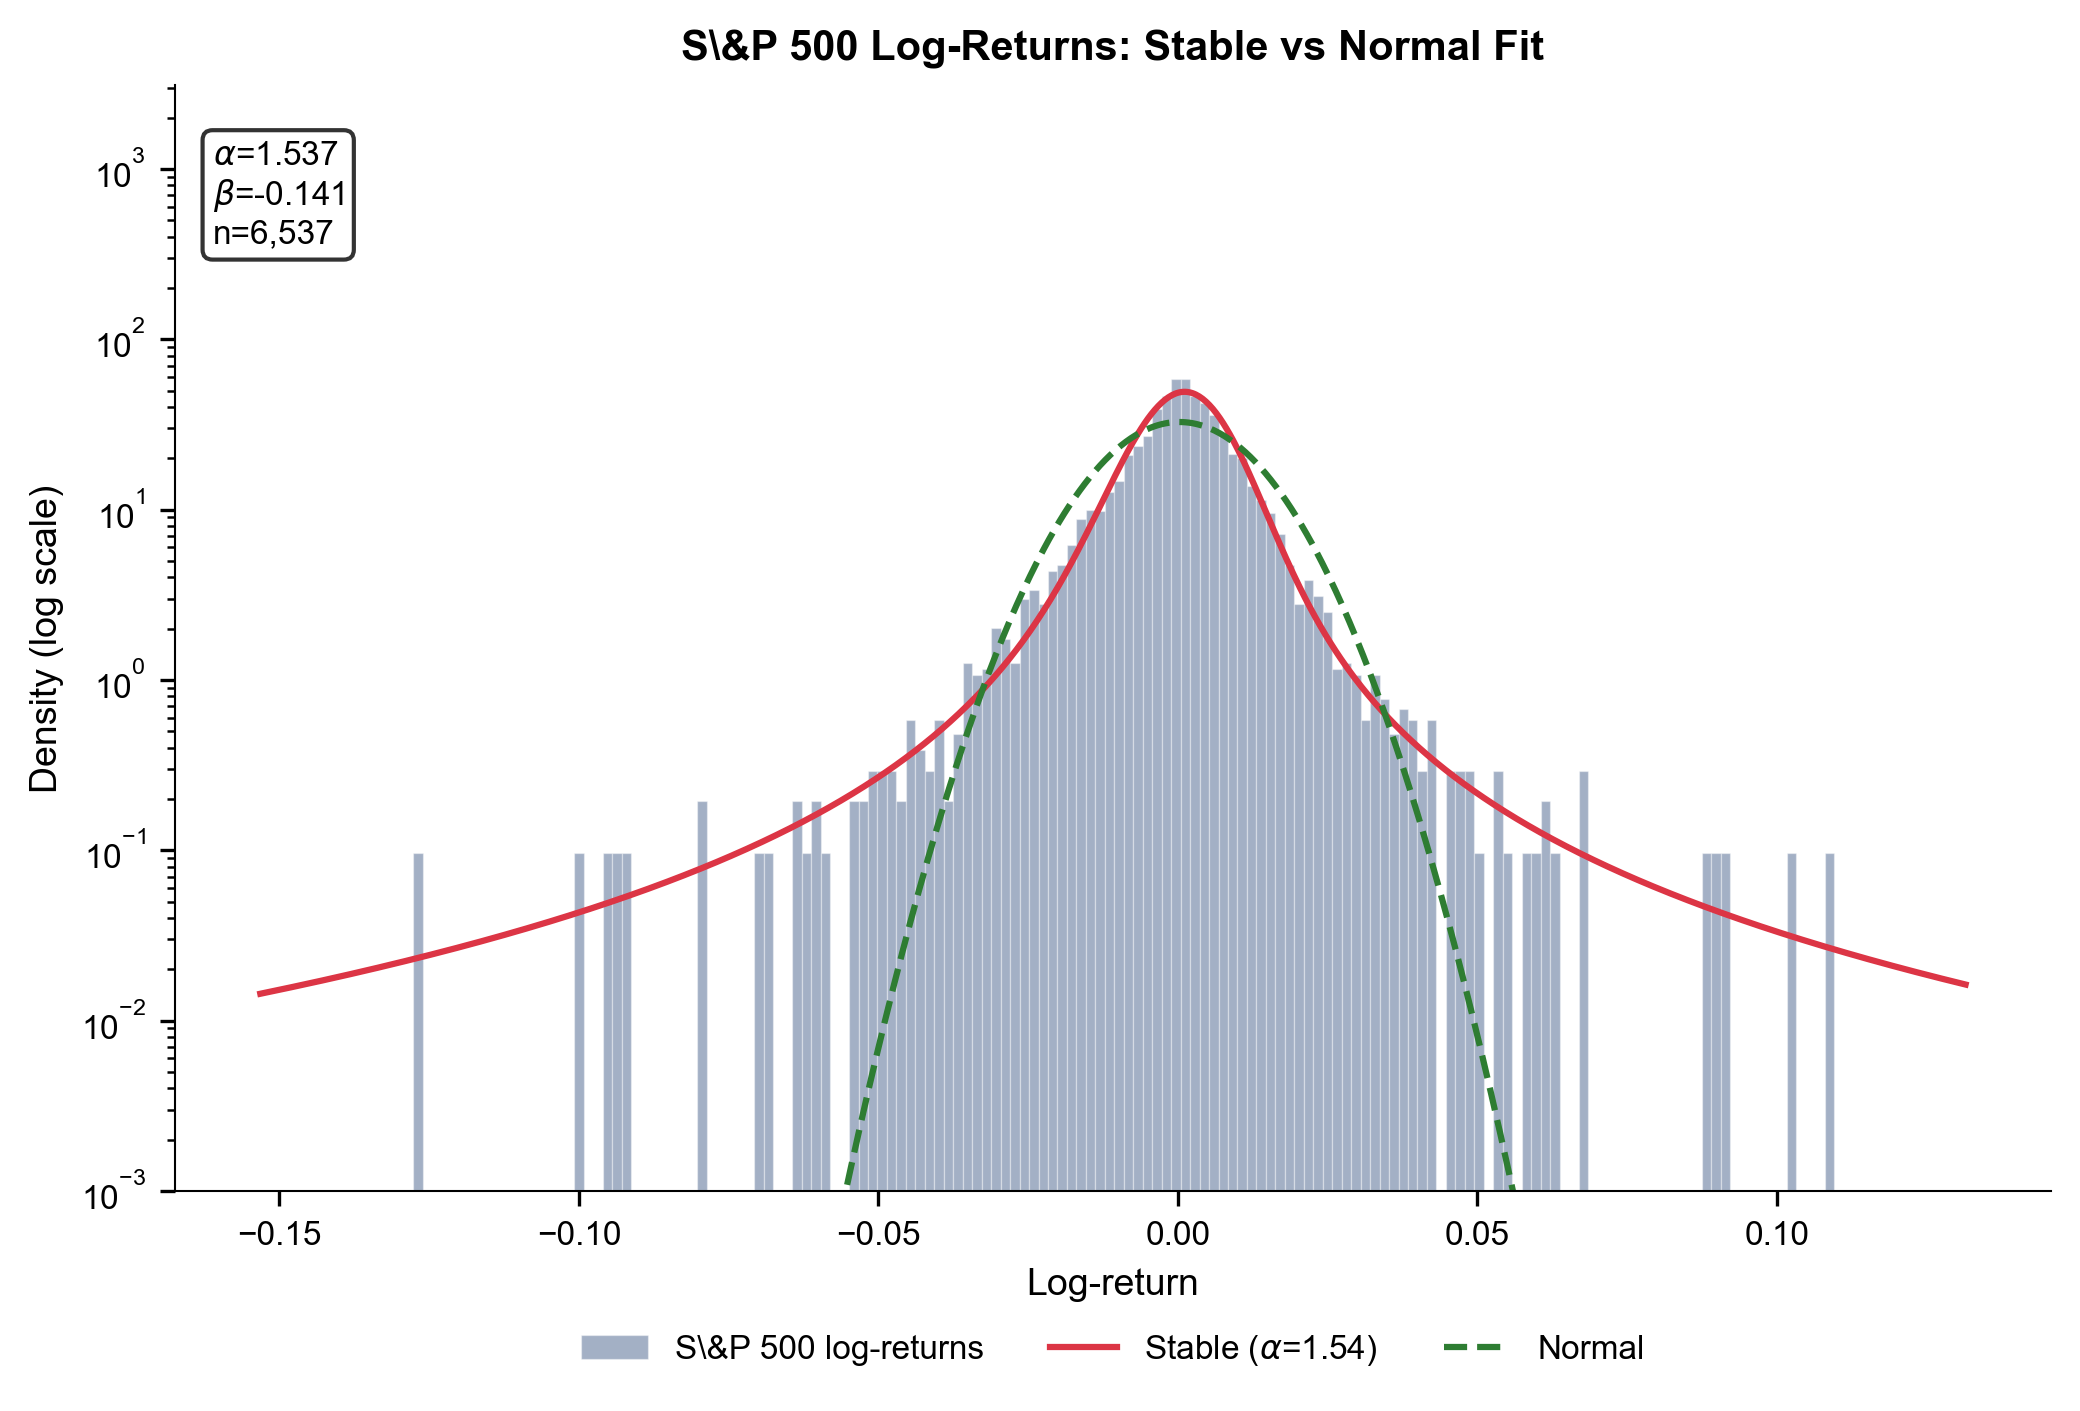
\includegraphics[width=0.85\textwidth]{ch2_sp500_stable_fit.png}
\end{center}

\vspace{-0.2cm}
\begin{itemize}
    \item Distribuția stabilă se potrivește mai bine în \textbf{centru} și în \textbf{cozi}
    \item Normala supraestimează densitatea la $\pm 1\sigma$ și subestimează în cozi
\end{itemize}
\end{frame}

\begin{frame}{Comparație PDF pe scară logaritmică}
\quantlet{SFM\_ch2\_stable\_fit}{https://github.com/QuantLet/SFM}

\begin{columns}[T]
\begin{column}{0.55\textwidth}
\begin{center}
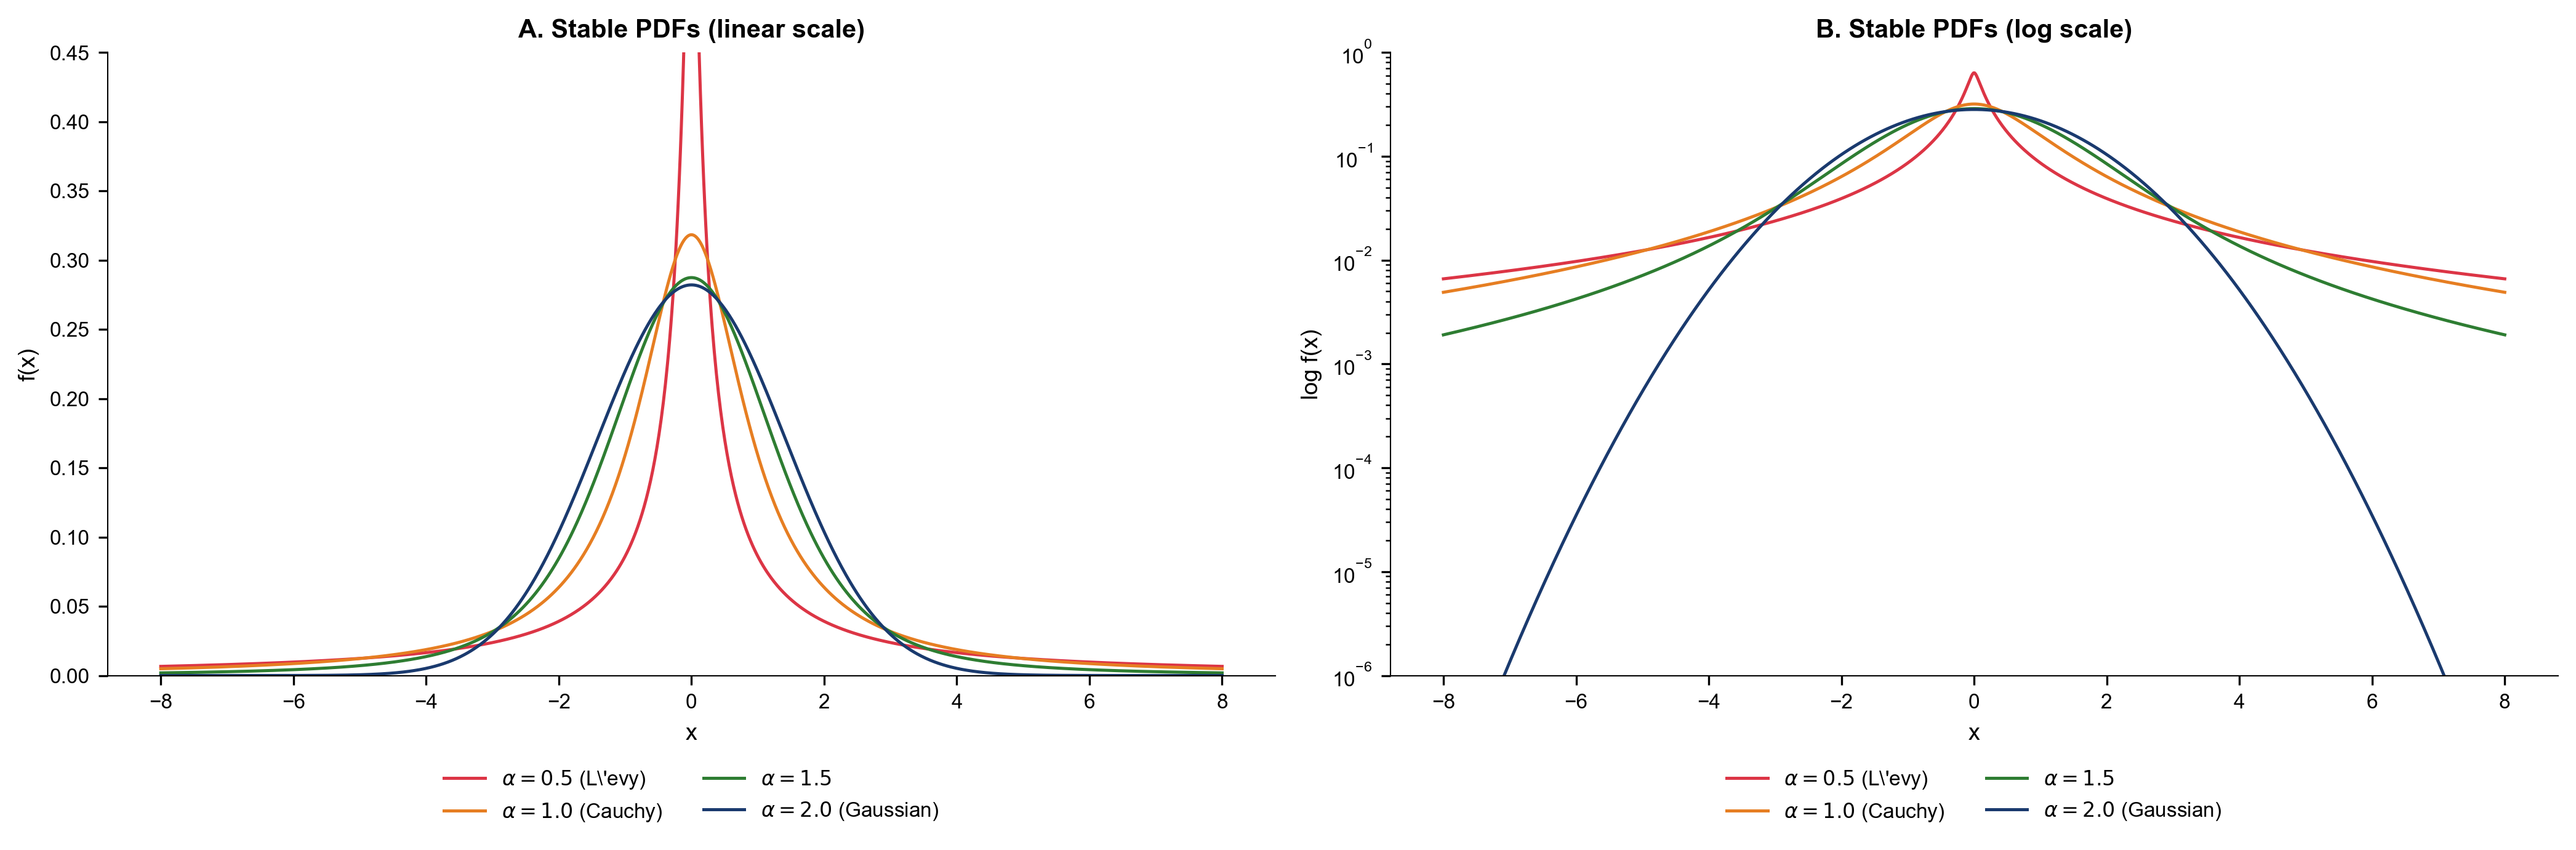
\includegraphics[width=\textwidth]{ch2_stable_pdfs.png}
\end{center}
\end{column}
\begin{column}{0.42\textwidth}
\textbf{Observații:}
\begin{itemize}
    \item Panoul B (scară log) evidențiază diferențele din cozi
    \item Distribuția cu $\alpha = 0.5$ (L\'{e}vy) are cele mai grele cozi
    \item La $\alpha = 2.0$ se obține exact distribuția normală
    \item Randamentele financiare au de regulă $\alpha \in [1.5, 1.9]$
\end{itemize}
\end{column}
\end{columns}
\end{frame}

\begin{frame}{VaR: Tabel comparativ}
\begin{block}{VaR pe S\&P 500 (2000--2025): Gaussiană vs Stabilă vs Empiric}
\renewcommand{\arraystretch}{1.3}
\begin{center}
\begin{tabular}{lccc}
\toprule
\textbf{Nivel VaR} & \textbf{Gaussiană} & \textbf{Stabilă} & \textbf{Empiric} \\
\midrule
5\% & $-1.91\%$ & $-2.14\%$ & $-2.08\%$ \\
1\% & $-2.71\%$ & $-4.12\%$ & $-3.56\%$ \\
0.1\% & $-3.59\%$ & $-8.97\%$ & $-6.88\%$ \\
\bottomrule
\end{tabular}
\end{center}
\end{block}

\vspace{0.2cm}
\begin{itemize}
    \item La nivelul de 5\%, diferențele sunt mici
    \item La 1\%, modelul stabil este cu $\sim$50\% mai conservator decât Gaussiana
    \item La 0.1\%, modelul stabil estimează pierderi de \textbf{2.5$\times$} mai mari
    \item VaR-ul empiric se situează \textbf{între} cele două modele parametrice
\end{itemize}
\end{frame}

\begin{frame}{Comparație cross-asset: Indicele de stabilitate $\alpha$}
\quantlet{SFM\_ch2\_stable\_fit}{https://github.com/QuantLet/SFM}

\begin{center}
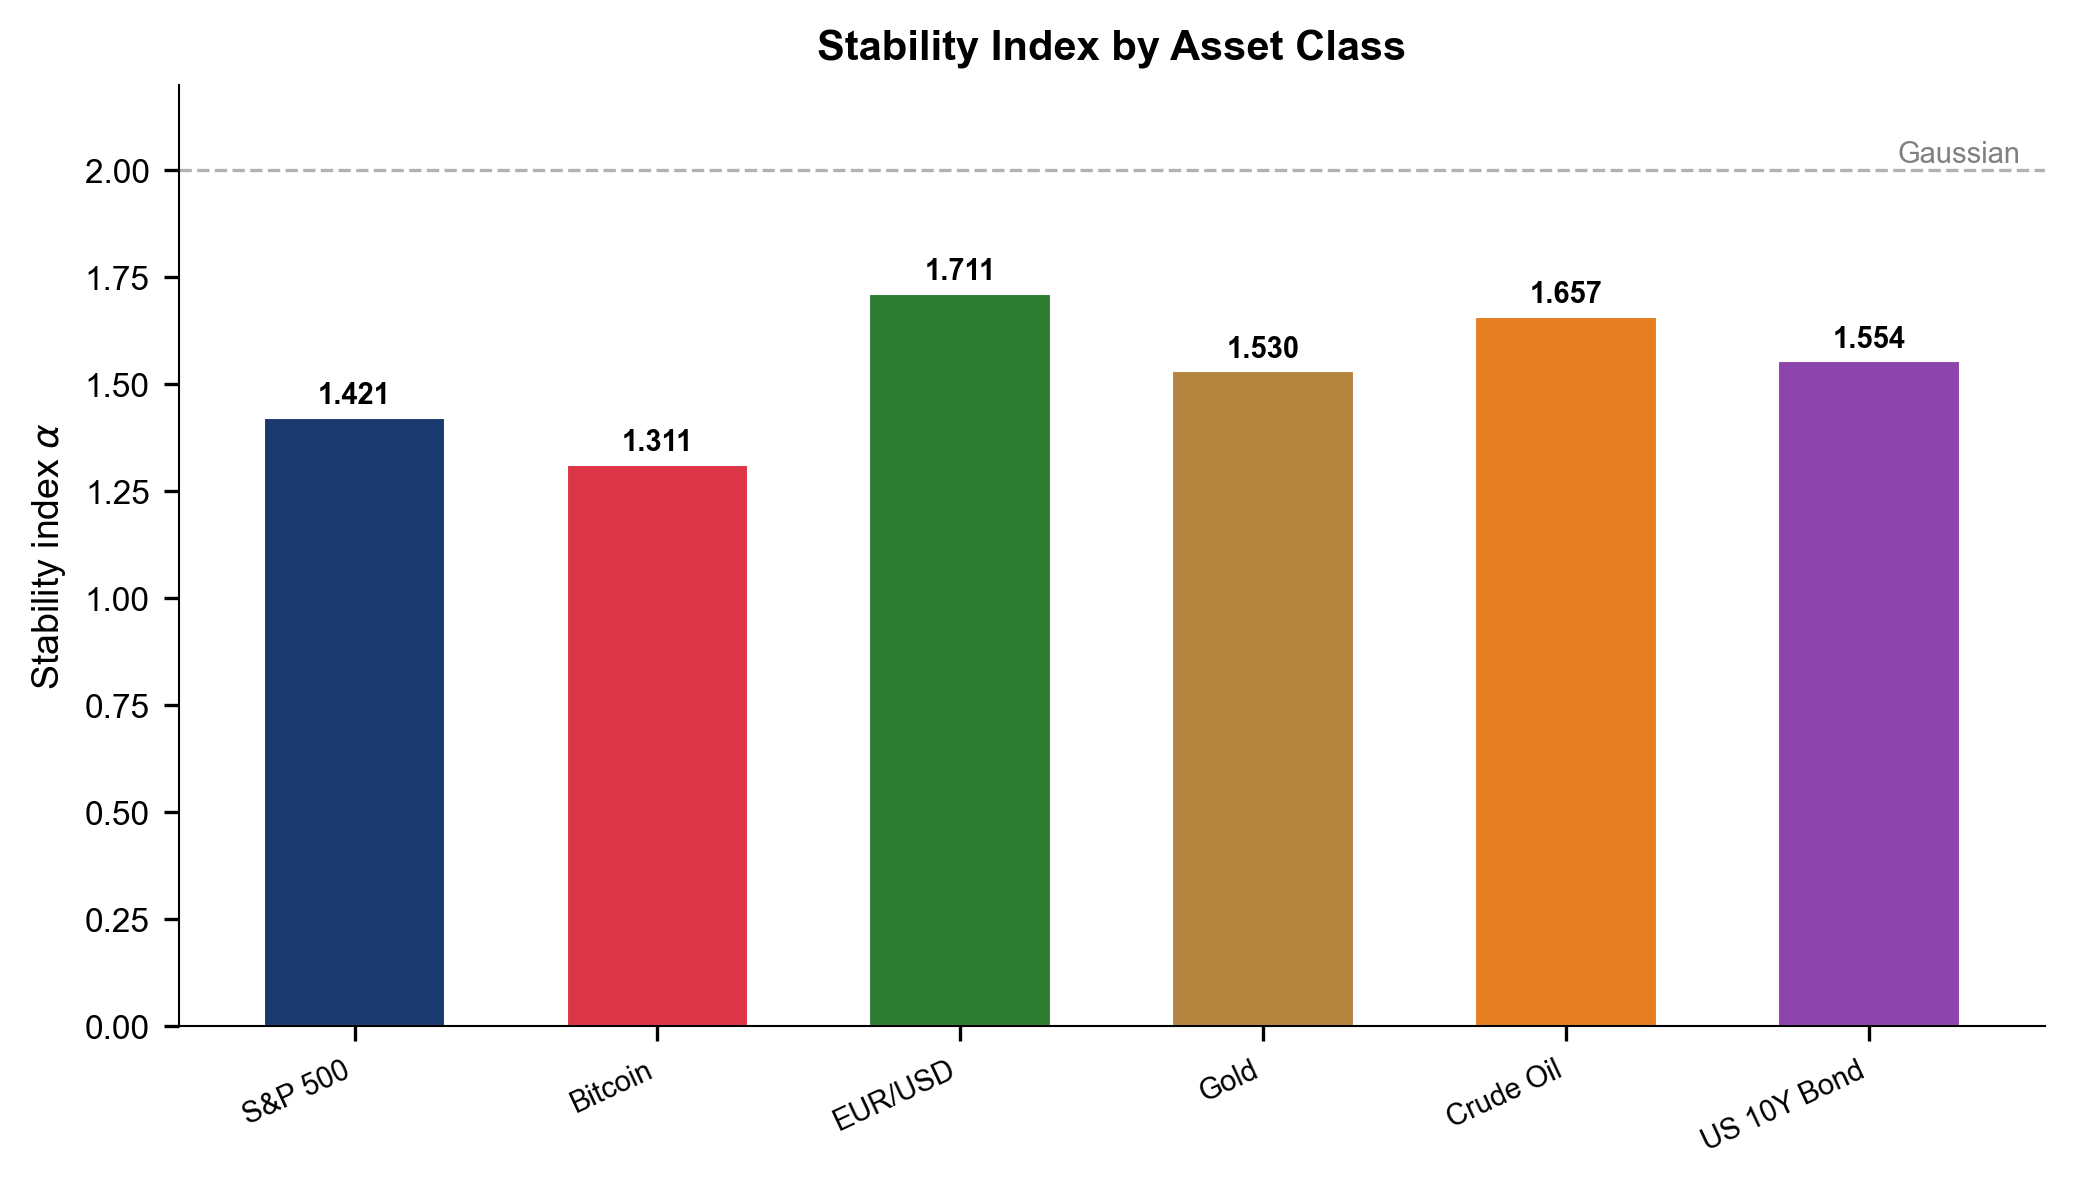
\includegraphics[width=0.75\textwidth]{ch2_cross_asset_alpha.png}
\end{center}

\vspace{-0.2cm}
\begin{itemize}
    \item Bitcoin are cel mai mic $\alpha$ $\Rightarrow$ cele mai grele cozi
    \item Obligațiunile au $\alpha$ cel mai mare (aproape Gaussian)
    \item \textbf{Nicio} clasă de active nu este perfect Gaussiană ($\alpha < 2$)
\end{itemize}
\end{frame}

%=============================================================================
% TEMĂ
%=============================================================================
\section{Tema pentru acasă}

\begin{frame}{Temă: Distribuții stabile pe BVB}
\begin{block}{Cerințe}
\begin{enumerate}
    \item Alegeți o acțiune listată la BVB (ex: TLV, SNP, BRD, FP)
    \item Descărcați datele zilnice din ultimii 5 ani
    \item Fit-ați o distribuție stabilă pe log-randamente
    \item Comparați grafic PDF stabilă vs normală (scară logaritmică)
    \item Calculați VaR la 1\% și 5\% (stabil vs normal vs empiric)
    \item Interpretați rezultatele: este piața românească ``mai Gaussiană'' decât S\&P 500?
\end{enumerate}
\end{block}

\vspace{0.2cm}
\begin{exampleblock}{Indicii}
\begin{itemize}
    \item Folosiți \texttt{yfinance} cu ticker-ul BVB (ex: \texttt{TLV.RO})
    \item Funcția \texttt{levy\_stable.fit()} poate fi lentă --- folosiți \texttt{floc=np.mean(data)}
    \item Comparați $\alpha$ estimat cu cel al S\&P 500
\end{itemize}
\end{exampleblock}
\end{frame}

%=============================================================================
% REZUMAT
%=============================================================================
\section{Rezumat}

\begin{frame}{Checklist competențe}
\begin{columns}[T]
\begin{column}{0.48\textwidth}
\begin{block}{Teorie}
\begin{itemize}
    \item[$\square$] Definiția stabilității prin sume
    \item[$\square$] Parametrii: $\alpha$, $\beta$, $\gamma$, $\delta$
    \item[$\square$] Cazuri speciale: Gauss, Cauchy, L\'{e}vy
    \item[$\square$] Funcția caracteristică
    \item[$\square$] Existența momentelor ($p < \alpha$)
    \item[$\square$] Comportamentul cozilor (lege putere)
\end{itemize}
\end{block}
\end{column}
\begin{column}{0.48\textwidth}
\begin{block}{Practică}
\begin{itemize}
    \item[$\square$] Estimarea McCulloch (cuantile)
    \item[$\square$] MLE cu \texttt{levy\_stable.fit()}
    \item[$\square$] Regresia Koutrouvelis (ECF)
    \item[$\square$] VaR: stabil vs normal vs empiric
    \item[$\square$] Simulare și vizualizare în Python
    \item[$\square$] Interpretarea $\alpha$ pe date reale
\end{itemize}
\end{block}
\end{column}
\end{columns}
\end{frame}

%=============================================================================
% PLANIFICAREA SEMINARELOR
%=============================================================================
\section{Planificarea seminarelor}

\begin{frame}{Planificarea seminarelor}
\renewcommand{\arraystretch}{1.3}
\begin{center}
\begin{tabular}{clll}
\toprule
\textbf{Săpt.} & \textbf{Tema} & \textbf{Curs asociat} & \textbf{Conținut principal} \\
\midrule
1 & Randamente & Cap. 1: Surse de date & Tipuri randamente, staționaritate \\
\rowcolor{MainBlue!10}
\textbf{2} & \textbf{Distribuții stabile} & \textbf{Cap. 2: Distribuții} & \textbf{Fit stabil, VaR, cozi grele} \\
3 & EMH \& Random Walk & Cap. 3--4 & Teste EMH, variance ratio \\
4 & Fapte stilizate & Cap. 5--6 & ACF, clustering volatilitate \\
\bottomrule
\end{tabular}
\end{center}
\end{frame}

%=============================================================================
% TEST RAPID
%=============================================================================
\section{Test rapid}

\begin{frame}{Quiz: 5 întrebări}
\begin{enumerate}
    \item Care sunt limitele parametrului de stabilitate $\alpha$?
    \begin{enumerate}
        \item[(a)] $0 < \alpha \leq 1$
        \item[(b)] $0 < \alpha \leq 2$
        \item[(c)] $-2 \leq \alpha \leq 2$
        \item[(d)] $\alpha > 0$
    \end{enumerate}

    \vspace{0.2cm}
    \item Pentru o distribuție $S(1.6, 0, 1, 0)$, care momente \textbf{există}?
    \begin{enumerate}
        \item[(a)] Media și varianța
        \item[(b)] Doar media
        \item[(c)] Toate momentele
        \item[(d)] Niciun moment
    \end{enumerate}

    \vspace{0.2cm}
    \item Ce distribuție se obține la $\alpha = 1, \beta = 0$?
    \begin{enumerate}
        \item[(a)] Gaussiană
        \item[(b)] Cauchy
        \item[(c)] L\'{e}vy
        \item[(d)] Exponențială
    \end{enumerate}
\end{enumerate}
\end{frame}

\begin{frame}{Quiz: 5 întrebări (cont.) + Răspunsuri}
\begin{enumerate}
    \setcounter{enumi}{3}
    \item În metoda McCulloch, $v_\alpha = 2.44$ corespunde:
    \begin{enumerate}
        \item[(a)] Cauchy
        \item[(b)] Gaussiană
        \item[(c)] L\'{e}vy
        \item[(d)] Stabil($\alpha = 1.5$)
    \end{enumerate}

    \vspace{0.2cm}
    \item De ce VaR stabil $>$ VaR Gaussian la 0.1\%?
    \begin{enumerate}
        \item[(a)] Distribuția stabilă are cozi mai grele
        \item[(b)] Distribuția stabilă este mai simetrică
        \item[(c)] Gaussiana are varianță infinită
        \item[(d)] Parametrul $\beta$ este negativ
    \end{enumerate}
\end{enumerate}

\vspace{0.3cm}
\begin{exampleblock}{Răspunsuri}
\begin{enumerate}
    \item \textbf{(b)} $0 < \alpha \leq 2$
    \item \textbf{(b)} Doar media (deoarece $p < \alpha = 1.6$, deci doar $p < 1.6$)
    \item \textbf{(b)} Cauchy
    \item \textbf{(b)} Gaussiană ($\alpha = 2.0$)
    \item \textbf{(a)} Cozile mai grele ale distribuției stabile
\end{enumerate}
\end{exampleblock}
\end{frame}

%=============================================================================
% BIBLIOGRAFIE
%=============================================================================
\section{Bibliografie}

\begin{frame}{Referințe}
\begin{thebibliography}{9}
\setbeamertemplate{bibliography item}[text]

\bibitem{nolan2020}
J.P. Nolan, \textit{Stable Distributions: Models for Heavy Tailed Data}, Birkh\"{a}user, 2020.

\bibitem{mandelbrot1963}
B. Mandelbrot, ``The variation of certain speculative prices,'' \textit{Journal of Business}, 36(4), 1963.

\bibitem{rachev2003}
S.T. Rachev, S. Mittnik, \textit{Stable Paretian Models in Finance}, Wiley, 2000.

\bibitem{franke2019}
J. Franke, W.K. H\"{a}rdle, C.M. Hafner, \textit{Statistics of Financial Markets}, 4th ed., Springer, 2019.

\bibitem{mcculloch1986}
J.H. McCulloch, ``Simple consistent estimators of stable distribution parameters,'' \textit{Communications in Statistics --- Simulation and Computation}, 15(4), 1986.

\end{thebibliography}

\vspace{0.3cm}
\textbf{Resurse online:}
\begin{itemize}
    \item \url{https://quantlet.com} --- Quantlet repository
    \item \url{https://danpele.github.io/SFM/} --- Materialele cursului
\end{itemize}
\end{frame}

%=============================================================================
% MULȚUMESC
%=============================================================================
{
\setbeamertemplate{headline}{}
\setbeamertemplate{footline}{}
\begin{frame}{}
    \centering

    \Huge\textcolor{MainBlue}{Mulțumesc!}

    \vspace{0.8cm}

    \Large Întrebări?

    \vspace{1cm}

    \normalsize
    Materialele cursului: \url{https://danpele.github.io/SFM/}

    \vspace{0.3cm}

    \href{https://quantlet.com}{\raisebox{-0.15em}{
\includegraphics[height=0.8em]{ql_logo.png}} Quantlet}
    \hspace{0.5cm}
    \href{https://quantinar.com}{\raisebox{-0.15em}{
\includegraphics[height=0.8em]{qr_logo.png}} Quantinar}
\end{frame}
}

\end{document}
